%%%%%%%%%%%%%%%%%%%%%%%%%%%%%%%%%%%% Chapter Template

\chapter{Introduction} 	% Main chapter title
\label{Introduction} 		% For referencing the chapter elsewhere, usage \ref{Introduction}

%%%%%%%%%%%%%%%%%%%%%%%%%%%%%%%%%%%% SECTION 1

\section{Ozone Kitesurf}
\label{sec:In1.1}

Ozone is one of the world’s leading manufacturers of Kites and Paragliders, created around a dedicated team of passionate riders and pilots that share the same outstanding passion for nature, exciting sports and progress.

\begin{wrapfigure}{r}{0.6\textwidth}
\centering
    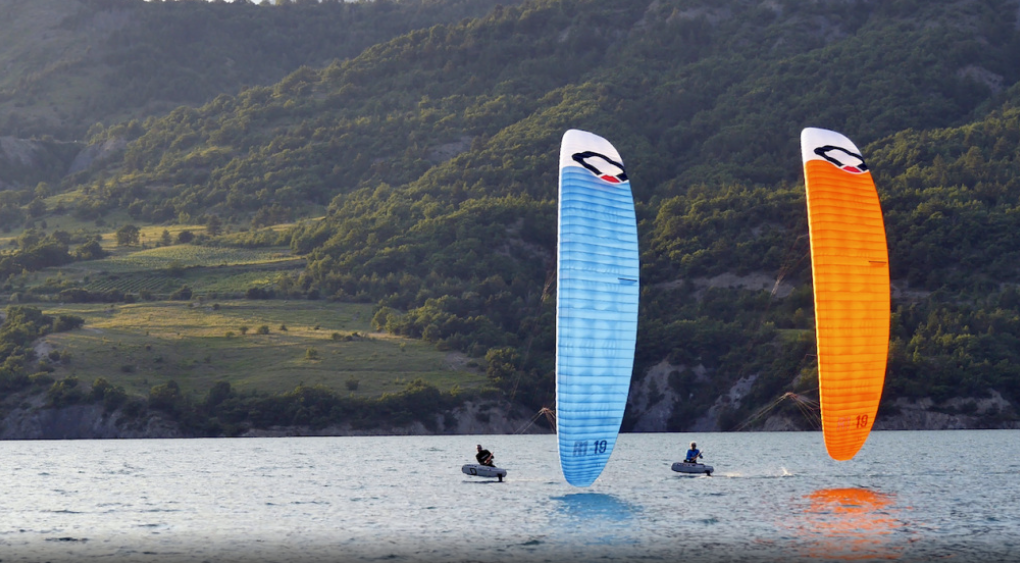
\includegraphics[width=0.6\textwidth]{figures/introduction/two_ozone_kite.png}
    \caption{Two Ozone racing kites}
    \label{fig:Two_Ozone_racing_kite}
\end{wrapfigure}

%Keeping true to their philosophy of creating products that they love to use, we extend that same passion into every aspect of the brand, working hard to innovate not only the products they create but also in their business practice and manufacturing process.

%they are proud of what they do and of who they are. Their core mission is to progress their sport through technological innovation, intensive R\&D and sustainable business models.

Their products conjure an experience that is nearly impossible to put into words. Invoking emotion, excitement, exhilaration and joy, the Ozone ‘feeling’ is something that transcends the product itself.

The Ozone factory in Vietnam is a state of the art facility were they employ only the highest trained craftsman whose expertise and attention to detail shine through in every product that is manufactured. their factory produces exclusively for Ozone Kites, Ozone Paragliders, Ozone Speedwings and Squirrel Wingsuits.

All Ozone products are checked and batch tested throughout the manufacturing process and must pass final checks before they leave the factory. Close contact between their product development teams and production facility ensures that every product is manufactured to specifications and is guaranteed to be worthy of the Ozone name.

They do not produce in large batches; all products are manufactured to order using their bespoke B2B ordering system. This method of production is unique to the Kitesurf industry, and means there is no extra stock flooding into the market, which can devalue a product at the end of the season.

Since the development of their very first kite in 2001, Ozone has brought more innovative concepts and industry leading designs to market than any other brand while creating category-defining products that set the standard for all those that follow.

They believe strongly in investing in tools that allow their team to advance designs with high efficiency and accuracy. They have developed their own proprietary software OzCAD by collaborating with some of the most brilliant minds in the fields of engineering, aerodynamics and software development.

Ozone has created the Version Concept for all products rather than confining them to model years. Designs are updated to a new version when they believe they have developed a better performing product from the existing design.

They have adopted this approach to avoid confusion in model updates; this also gives their design team time for true innovation \cite{ozonekites}.

%%%%%%%%%%%%%%%%%%%%%%%%%%%%%%%%%%%% SECTION 2

\section{The Ozone design team}
\label{sec:In1.2}

\begin{figure}[H]
    \centering
    \includegraphics[width=1\textwidth]{figures/introduction/Ozone team présentation.png}
    \caption{The Ozone design team involved in this internship}
    \label{fig:The Ozone design team}
\end{figure}

Ozone provided me with the opportunity to work with a myriad of highly skilled and passionate kitesurfing professionals.

The kite design team is composed of :
\begin{itemize}
    \item \textbf{Dominik Zimmermann} : head designer and foil tester
    \item \textbf{Rob Whittall} : product designer, co owner and co founder of Ozone and ex-world paragliding and hang gliding champion
    \item \textbf{Simon Burner} : assistant designer and test rider
    \item \textbf{Torrin Bright} : product manager and test rider
\end{itemize}

Additionally, throughout the internship, I had frequent interactions with the Ozone paraglider design team. Due to the significant overlap in aerodynamics between these two fields, I was able to leverage their expertise and experience. \textbf{Luc Armand} and \textbf{Fred Pieri}, research and development engineers and experienced pilots, provided valuable support for my research efforts in developing a Python-based optimization algorithm for their upcoming paraglider design.

Furthermore, \textbf{Axel Mazella}, a member of the racing team, two-time Kitefoil World Champion and European Champion, provided me with valuable feedback and insights from his testing of our prototypes. This input helped me better understand the optimization challenges in kite design and bridge the gap between the scientific aspects and the practical realities of kite riding.

%%%%%%%%%%%%%%%%%%%%%%%%%%%%%%%%%%%% SECTION 3

\section{The Olympic Games}
\label{sec:In1.3}

The 2024 Olympic Games will introduce kitesurfing for the first time, encompassing various disciplines.

As the name implies, athletes are propelled across the water's surface while holding a 7-21m kite to harness the power of the wind.

In many respects, it represents a fusion of water sports. Competitors need the balance of a surfer while reaching speeds similar to those in windsurfing, using equipment that closely resembles a wakeboard.

When the wind is strong enough, riders can achieve speeds of up to 40 knots (74 km/h) and have been observed soaring up to six meters in the air \cite{olympics}.

% \begin{wrapfigure}[9]{l}{0.6\textwidth}
% \centering
%     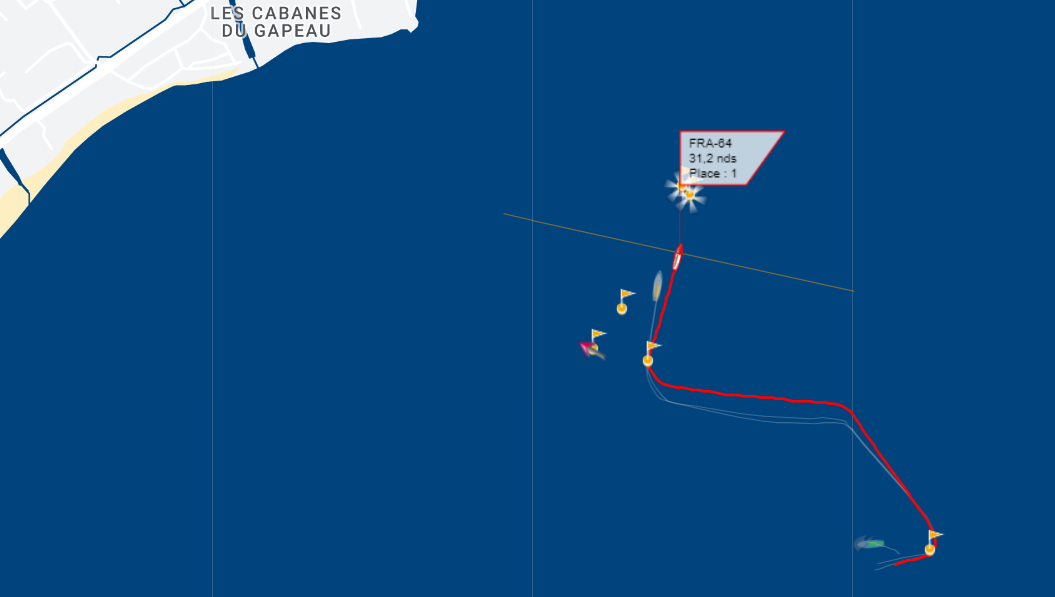
\includegraphics[width=0.6\textwidth]{figures/introduction/suivi_course_kite_axel.png}
%     \caption{Example of a trajectory during a kite race}
%     \label{fig:Example_of_a_trajectory_during_a_kite_race}
% \end{wrapfigure}

Races are typically conducted as short-course, windward-leeward races. The number of races, race format, and course length may vary depending on the event and conditions. They begin with a starting sequence involving flags, signals, and countdowns then, the athletes must reach buoys to complete the race.
\vspace{3cm}

The class features a foil kite and a board with a hydrofoil. The equipment is not one-design, but instead competitors use their choice of approved production equipment. The International Kiteboarding Association (IKA) manages the class \cite{formula_kite}.

\begin{figure}[H]
    \centering
    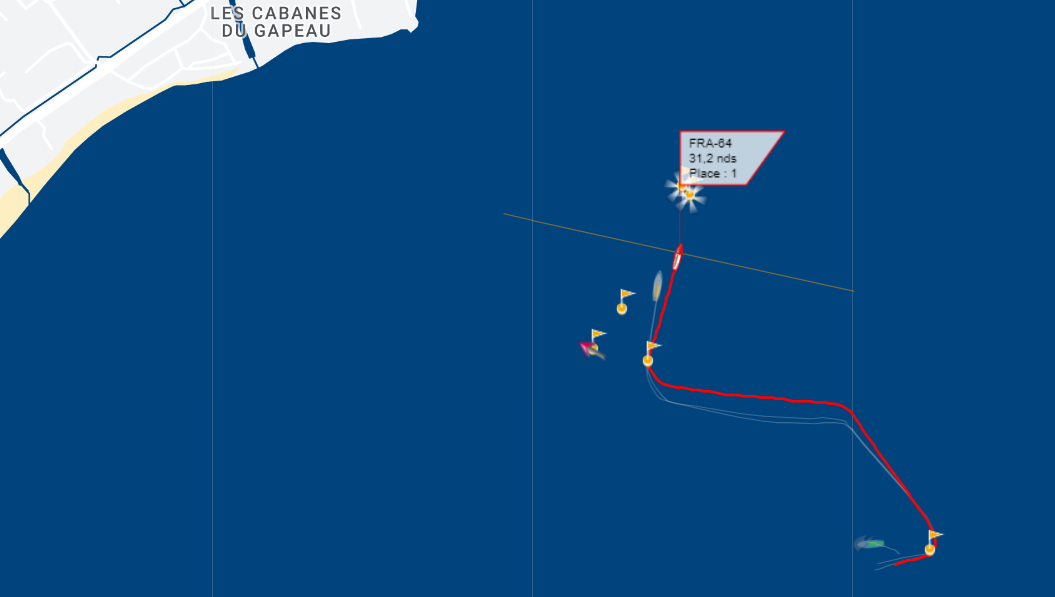
\includegraphics[width=1.\textwidth]{figures/introduction/suivi_course_kite_axel.png}
    \caption{Example of a trajectory followed during a kite race.}
    \label{fig:Example_of_a_trajectory_during_a_kite_race}
\end{figure}

%%%%%%%%%%%%%%%%%%%%%%%%%%%%%%%%%%%% SECTION 4

\section{The Ozone R1V4 formula kite}
\label{sec:In1.4}

The current formula kite used by Ozone in the Olympic Games is the R1V4.

However, it faces stiff competition from a more efficient rival, the Flysurfer "VMG". This was the primary objective of the internship: to develop the fifth iteration of the R1 kite, known as the "R1V5," in preparation for the 2028 Olympic Games. 

With the registration deadline set for March 2024, there was a very real time constraint in the design of the kite..

\begin{figure}[H]
    \centering
    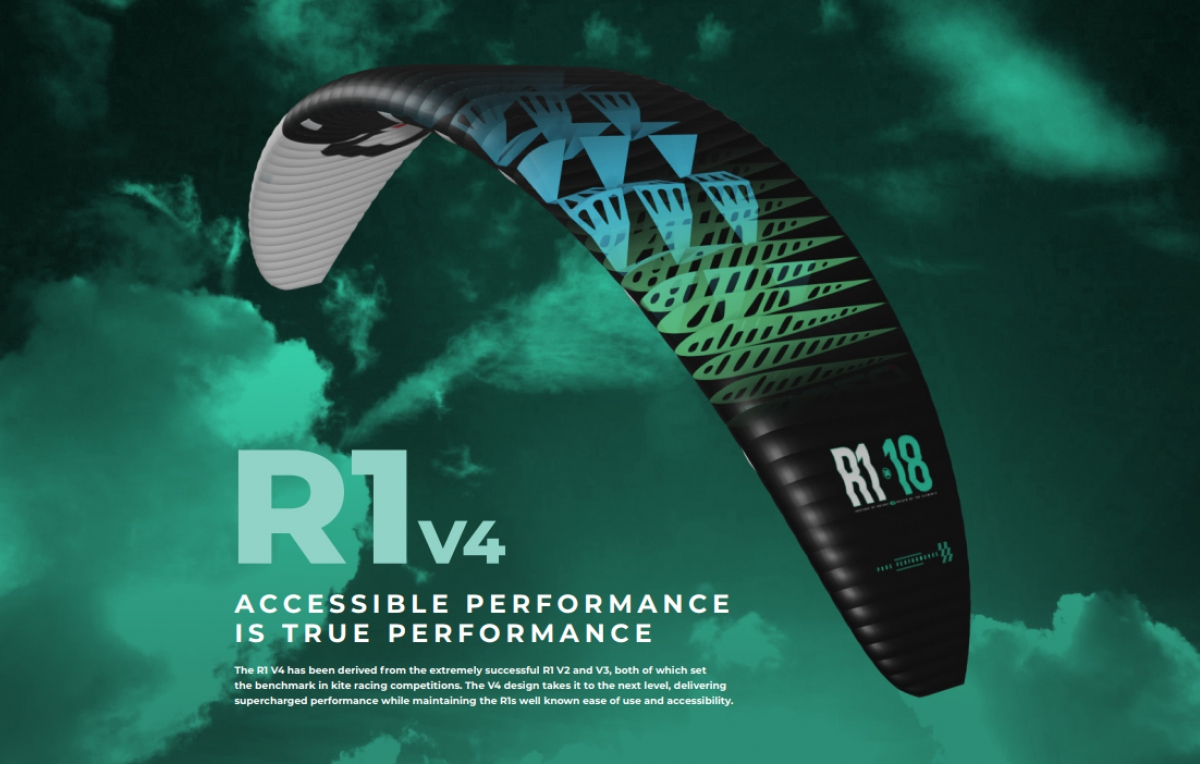
\includegraphics[width=1.\textwidth]{figures/introduction/R1V4.jpg}
    \caption{The Ozone R1V4 formula kite}
    \label{fig:R1V4}
\end{figure}